\documentclass[10pt]{amsart}
\usepackage[margin=1.4in]{geometry}
\usepackage{amssymb,amsmath,enumitem,url}
\usepackage{graphicx,subfig}
\graphicspath{ {./images/} }

\newcommand{\D}{\mathrm{d}}
\newcommand{\I}{\mathrm{i}}
\DeclareMathOperator{\E}{e}
\DeclareMathOperator{\OO}{O}
\DeclareMathOperator{\oo}{o}
\DeclareMathOperator{\erfc}{erfc}
\DeclareMathOperator{\real}{Re}
\DeclareMathOperator{\imag}{Im}
\usepackage{tikz}
\usepackage[framemethod=tikz]{mdframed}
\theoremstyle{nonumberplain}

\mdtheorem[innertopmargin=-5pt]{sol}{Solution}
%\newmdtheoremenv[innertopmargin=-5pt]{sol}{Solution}

\begin{document}
\pagestyle{empty}

\newcommand{\mline}{\vspace{.2in}\hrule\vspace{.2in}}

\noindent
\text{Hunter Lybbert} \\
\text{Student ID: 2426454} \\
\text{03-13-25} \\
\text{AMATH 502} \\
% header containing your name, student number, due date, course, and the homework number as a title.

\title{\bf {Homework 8} }


\maketitle
\noindent
Exercises come from the assignment sheet provided by the professor on canvas.
\mline
\begin{enumerate}[label={\bf {\arabic*}:}]
\item See assignment document for background on the \textit{Sierpinski Carpet}.
\begin{enumerate}

\item Show that the (Lebesgue) measure of the resulting fractal is 0.
Justify your work. \\

\textit{Solution:} \\
Notice the following pattern in the measure (or area in this case) of each step denoted as $S_n$:
\begin{align*}
S_0 &= 1 = \left( 8/9 \right)^0\\
S_1 &= 1 \cdot \frac 8 9  = \left( \frac 8 9 \right)^1 \\
S_2 &= \sum_{i=1}^8\frac 1 9 \cdot \frac 8 9  = \left( \frac 8 9 \right)^2 \\
&\vdots \\
S_n &= \left( \frac 8 9 \right)^n.
\end{align*}
Finally, the limiting set forming the fractal of interest $S_\infty$ has measure 0 since
$$\lim_{n\rightarrow\infty} \left( \frac 8 9 \right)^n = 0.$$
\qed \\

\item Find the similarity dimension of the limiting fractal. Show and explain your work. \\

\textit{Solution:} \\
Following the examples in Strogatz we define the similarity dimension of the limiting fractal to be
\begin{equation}
d = \frac {\ln m}{\ln r}
\label{eq:sim_dim}
\end{equation}
where $m$ is the number of copies and $r$ is the scale factor of the fractal.
In our particular fractal we have $m = 8$ and $r = 3$.
Therefore, our similarity dimension for this carpet fractal is 
$$
d = \ln 8/\ln 3
$$
\qed \\

\item Show that the box-counting dimension of this fractal is the same as the similarity dimension. (You may not be able to complete this until box-counting dimension is defined in class). \\

\textit{Solution:} \\
Notice, that by definition of the box counting dimension is
\begin{equation}
d = \lim_{\epsilon \rightarrow 0} \frac {\ln N(\epsilon)}{\ln (1/\epsilon)}.
\label{eq:box_dim}
\end{equation}
Now for this carpet fractal, each $S_n$ consists of $8^n$ squares with side length $(1/3)^n$.
So if we pick $\epsilon = (1/3)^n$ we need all $8^n$ of these squares to cover this carpet fractal.
Hence $N = 8^n$ when $\epsilon = (1/3)^n$.
Since $\epsilon \rightarrow 0$ as $n \rightarrow \infty$, we have the boxing dimension of
$$
d = \lim_{\epsilon \rightarrow 0} \frac {\ln N(\epsilon)}{\ln (1/\epsilon)}
	= \frac {\ln (8^n)}{\ln (3^n)}
	= \frac {n \ln 8}{n \ln 3}
	= \frac {\ln 8 }{\ln 3}.
$$
Which is exactly what we got for the similarity dimension. \\
\qed \\

\item Show that there are uncountably many points on the interior of the limiting fractal (i.e. infinitely many points without x = 0, x = 1, y = 0, or y = 1). \\
\textbf{Hint:} Try showing this in just one dimension, e.g., show that there are uncountably many points (x, y) with a fixed value of y, perhaps y = 0.5 is a good choice. \\

\textit{Solution:} \\
Notice, if we fix a value of $y = 0.5$, then the $x$ values in this cross section of the carpet fractal follow the pattern and sequence of the middle $1/3$ cantor set.
Citing example 11.2.3 from Strogatz, we know that the middle $1/3$ cantor set is uncountable, therefore the set of points in the fractal such that $x$ can vary and $y = 0.5$ are uncountable.
Since this is a subset of the limiting carpet fractal, then the whole set of points in the limiting fractal are uncountable. \\
\qed \\

\newpage

\end{enumerate}

\item In this problem we construct what is called a middle-halves Cantor set.
Consider the following Cantor set construction. Start with the interval [0, 1], then remove the middle half. Continue this process for each sub-interval. \\
\begin{enumerate}

\item Draw $S_1$ and $S_2$. \\

\textit{Solution:} \\
See Figure (\ref{fig:f1}).

\begin{figure}[h]
	\centering
	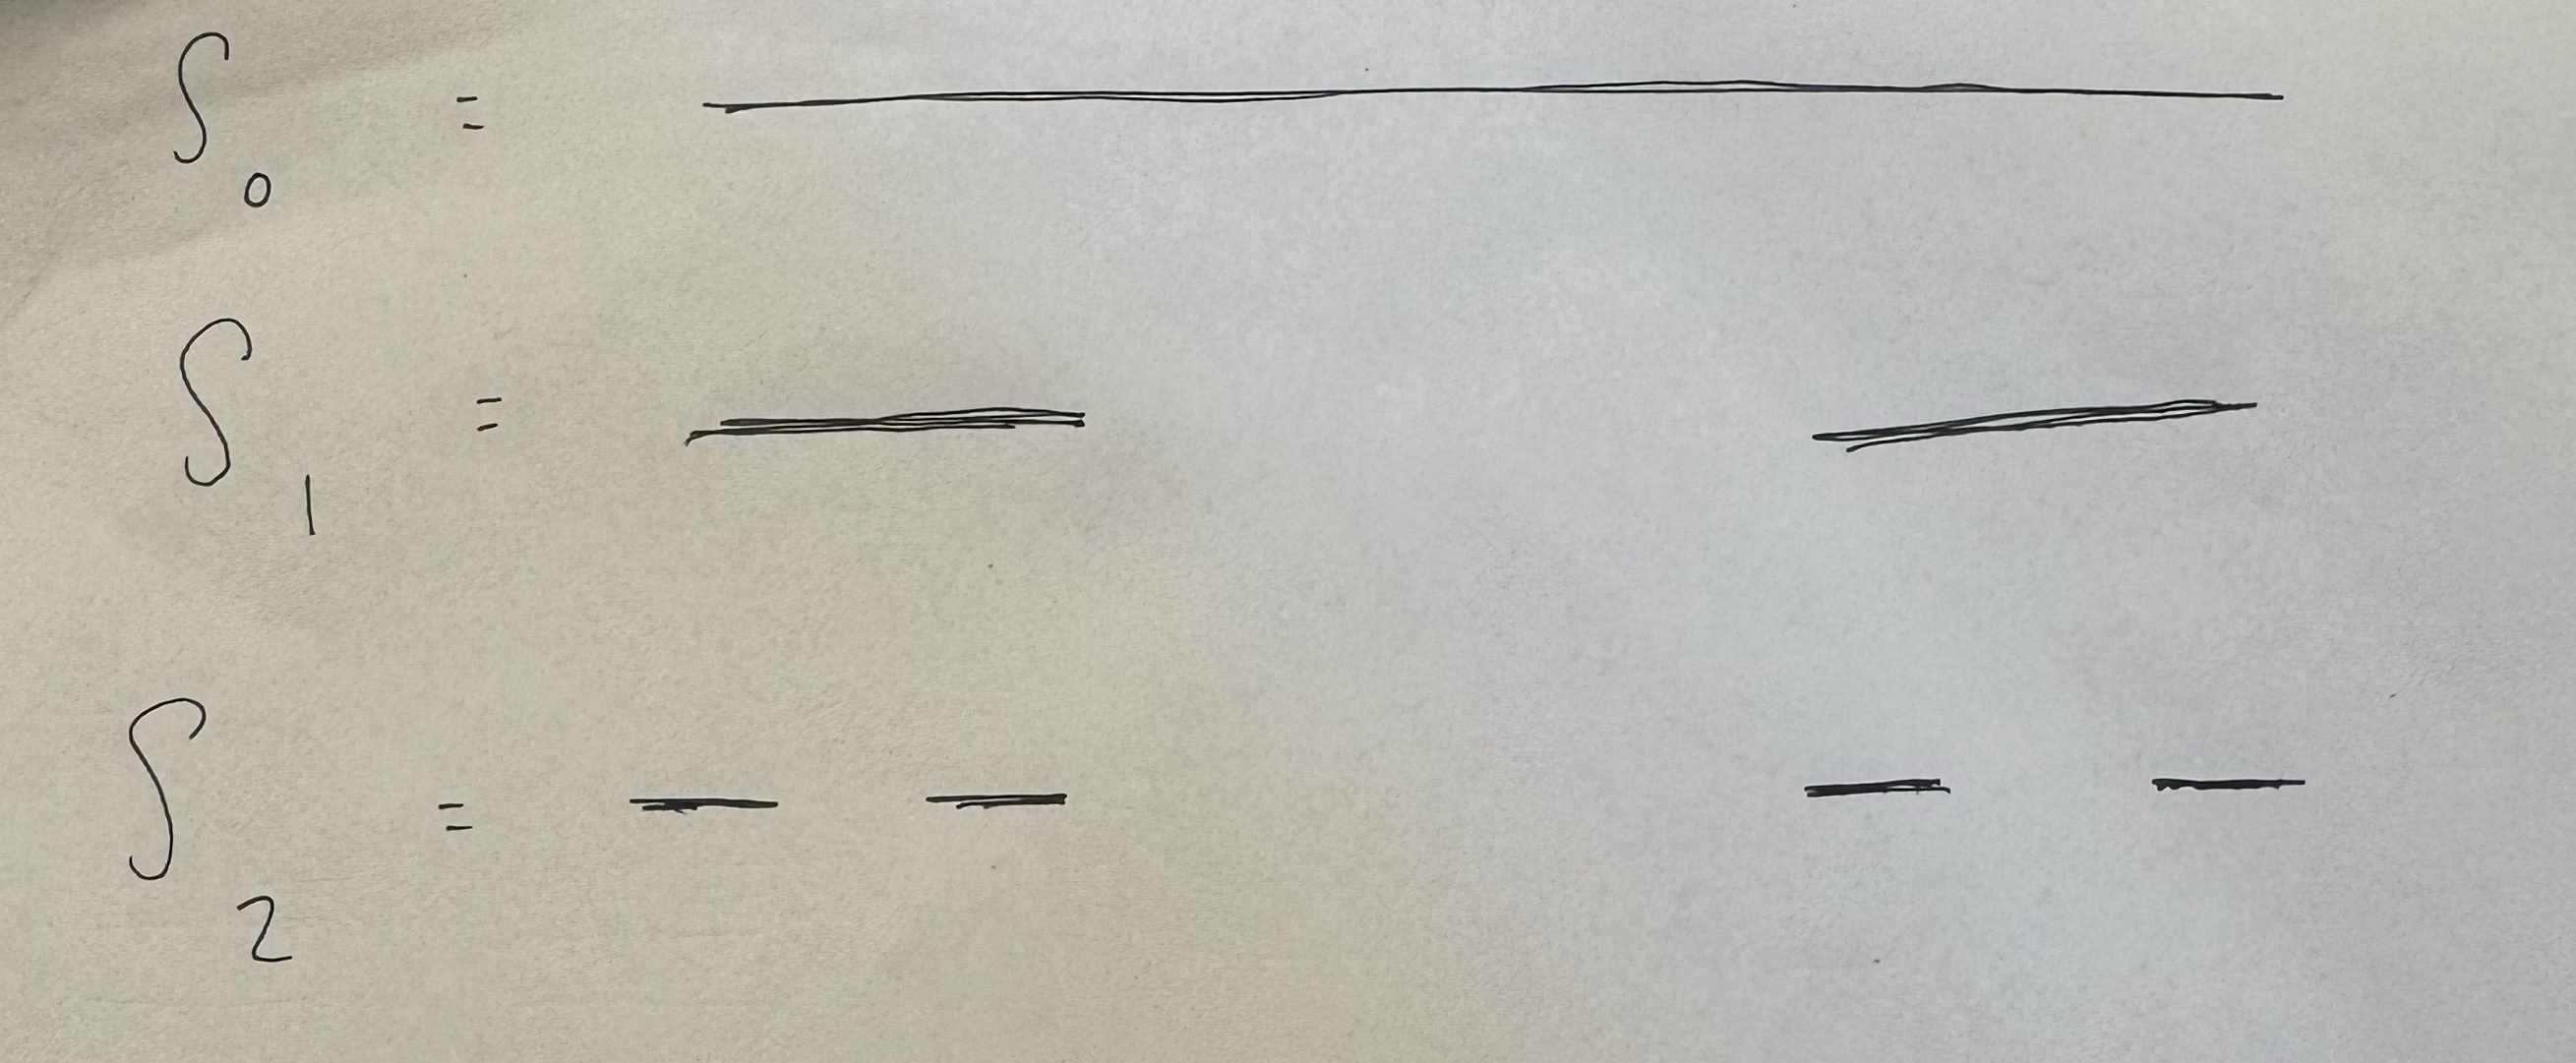
\includegraphics[height=.3\textwidth]{middle_half_cantor_set.png}
 	\caption{We have sketched the first 3 steps of the middle halves Cantor set.}\label{fig:f1}
\end{figure}
\qed \\

\item Find the similarity dimension of the set. \\

\textit{Solution:} \\
We have the number of copies $m = 2$ and the scale factor $r = 4$ therefore, using equation \eqref{eq:sim_dim} the similarity dimension is 
$$
d = \frac {\ln 2} { \ln 4}.
$$
\qed \\

\item Find the measure of the set. \\

\textit{Solution:} \\
Similar to problem 1 a), we can calculate the measure of the set as $S_n = (1/2)^n$ which leads to
$$
\lim_{n \rightarrow \infty} (1/2)^n = 0.
$$
\qed


\end{enumerate}

\newpage

\item See assignment sheet for details of the \textit{fat fractal}. \\

\begin{enumerate}
\item Find the (Lebesgue) measure of this cantor set. Show your work. \\

\textit{Solution:} \\
Let's do this by noting the measure of the unremoved line segment is 1, therefore the measure of the fat fractal will be $1 - R$, where $R$ is the total measure which is removed.
Notice, to go from the $n$ step to the $(n + 1)$th step we are removing a piece the size of $(2/7)^{n + 1}$ and we are removing $2^n$ of them.
Written in summation form this is
$$
R = \sum_{n = 0}^{\infty} 2^n(2/7)^{n + 1} = (2/7)\sum_{n = 0}^{\infty}(4/7)^{n} = (2/7) \frac 1 {1 - 4/7} = \frac 2 7 \frac 7 3 = 2/3
$$

where we used the geometric series with $r = 4/7$.
Therefore, the measure of the fat fractal is $1 - R = 1 - (2/3) = 1/3$. \\
\qed \\

\item Is the fractal self similar?
Justify your answer. \\
\textbf{Hint:} Can you find the similarity dimension of this set?
What happens when you try?) \\
\textbf{Note:} You may find this part to be difficult.
If you are struggling with it, you may want to skip it for now and come back to it later. 
\\

\textit{Solution:} \\
If we were to try and calculate the similarity dimension we need to calculate $m$, the number of additional copies we get each iteration and $r$ the scale factor for these new copies.
We can determine that $m$ is 2 in our case, however, the scale factor is not constant with so there is no one $r$ that works for all steps.
Therefore, the fat fractal is not self similar. \\
\qed \\

\end{enumerate}
 
\newpage
 
\item The tent map on the interval [0, 1] is defined by $x_{n + 1} = f(x_n)$, where 
$$
f(x) = \begin{cases}
rx,  &0 \leq x \leq \frac 1 2 \\
r(1 - x), &\frac 1 2 < x \leq 1
\end{cases}.
$$
Assume that $r > 2$.
Then some points get mapped outside of the interval [0, 1].
If $f(x_0) > 1$ then we say that $x_0$ has ``escaped" after one iteration.
Similarly, if $f^n(x_0) > 1$ for some finite $n$ and $n$ is the smallest integer for which this is true, then we say $x_0$ has escaped after $n$ iterations. \\
\textbf{Hint:} You should plot the function $f (x)$ and think about orbits of different initial
conditions when you are solving this problem, it will make your work much easier.
Use these plots to guide your analysis, the plots alone are not enough. \\

\begin{enumerate}
\item Find the set of initial conditions $x_0$ that escape after one iteration. \\

\textit{Solution:} \\
The set of initial conditions for which $x_0$ will escape in one iteration is all
$$
x_0 \in \left\{\frac 1 r < x \leq 1 - \frac 1 r \right\}.
$$
Now we calculated this by determining that any $x_0$ from in that range for example, the minimum $\frac 1 r$ we have $f(1/r) = r(1/r) = 1$ which is the lower bound for the output of the points in the set we have given.
It is easy and left to the reader to verify the upper bound as well. \\
\qed \\

\item Find the set of initial conditions $x_0$ that escape after two iterations. \\

\textit{Solution:} \\
Another way to state which $x_0$'s we are looking for is to say the set of $x_0$ which map to the set from part a) in one step.
And thus in the next iteration will escape in one (but two in total).
Essentially we are trying to find the pre-image of $\left\{\frac 1 r < x \leq 1 - \frac 1 r \right\}$ with respect to $f(x)$.
Using the example of $r = 3$, we see we are looking for the pre-image of $\left\{\frac 1 3 < x \leq \frac 2 3 \right\}$.
Notice, if $f(x) = 1/3$ we get $x = 1/9 \text{ or } 8/9$ and for $f(x) = 2/3$ we get $x = 2/7 \text{ or } 7/9$.
Hence,
$$
x_0 \in \left\{\frac 1 9 < x \leq \frac 2 9 \right\} \bigcup \left\{\frac 7 9 < x \leq \frac 8 9 \right\}
\implies
f(x_0) \in \left\{\frac 1 3 < x \leq \frac 2 3 \right\}.
$$
And thus $f(f(x_0)) \not \in [0, 1]$ and hence $x_0$ escaped in two steps.
Therefore, in general $r$ the set of initial conditions $x_0$ which escape in two steps exactly is
$$
x_0 \in \left\{\frac 1 r < x \leq \frac 1 r - \frac 1 {r^2} \right\}
\bigcup \left\{1 - \frac 1 r + \frac 1 {r^2} < x \leq 1- \frac 1 {r^2} \right\}.
$$
\qed \\


\item Describe the set of $x_0$ that never escape.
This is called the invariant set. \\
\textbf{Hint:} First look at what happens for $r = 3$.
Does this look like a set you recognize? \\

\textit{Solution:} \\
After inspecting this for $r = 3$ this is basically just the middle third Cantor set.
I could redraw that here, but that would be redundant at this point.
This set is quite interesting though, seeing as it has come up so many different ways in this homework assignment. \\
\qed \\

\item Find the box dimension of the invariant set (for general $r$, not $r = 3$). \\

\textit{Solution:} \\
The box dimension is going to be easy to calculate.
Using the setup from problem 1 c) and Equation (\eqref{eq:box_dim}) we can determine that in this case each step in the iteration consists of $2^n$ intervals which remain in the interval $[0, 1]$. 
Furthermore, if we pick $\epsilon = (1/r)^n$ we need all $2^n$ of these line segments to cover the ultimate fractal structure. 
Hence, $N(\epsilon) = 2^n$ and $\epsilon = (1/r)^n$.
Since $\epsilon \rightarrow 0$ as $n \rightarrow \infty$, we have the boxing dimension of
$$
d = \lim_{\epsilon \rightarrow 0} \frac {\ln N(\epsilon)}{\ln (1/\epsilon)}
	= \frac {\ln (2^n)}{\ln (r^n)}
	= \frac {n \ln 2}{n \ln r}
	= \frac {\ln 2 }{\ln r}.
$$
\qed \\

\end{enumerate}

\end{enumerate}

\end{document}

%%% Local Variables:
%%% mode: latex
%%% TeX-master: t
%%% End:
